\subsection{Pooling} \label{subs:pooling}
A Pooling layer replaces the input at a certain location with summary statistics of the inputs nearby \cite{goodfellow_deep_2016}. Pooling layers are inserted between the successive convolutional layer to modify the output further. It aims at reducing the spatial size of each \acrshort{fm} and making the representation invariant to small transitions. It also reduces the number of parameters and the computation of the network while also increasing the receptive field \cite{shawahna_fpga-based_2019}. The layer divides each \acrshort{fm} into regions of size $K \title K$ and outputs one pixel from each region. This way, we can keep the number of channels and reduce each spatial dimension by $K$.

Various pooling functions can be used, but the most common form is with filters of size $2 \times 2$ where the MAX or AVG operation selects the highest pixel from 4 samples (meaning a reduction 75\%) \cite{suda_throughput-optimized_2016}. An illustration can be found in figure \ref{fig:pool}.
%
\begin{figure}
    \centering
    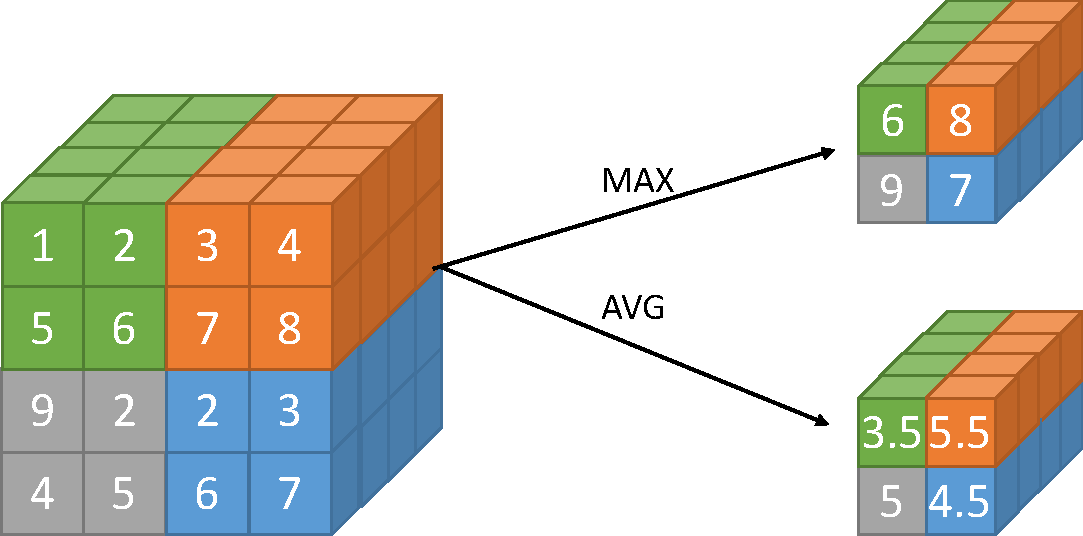
\includegraphics[width=\textwidth]{pooling.pdf}
    \caption{An example of pooling layers}
    \label{fig:pool}
\end{figure}
